\subsubsection{Search Available Tutors and Book sesion}
\begin{figure}[H]
    \centering
    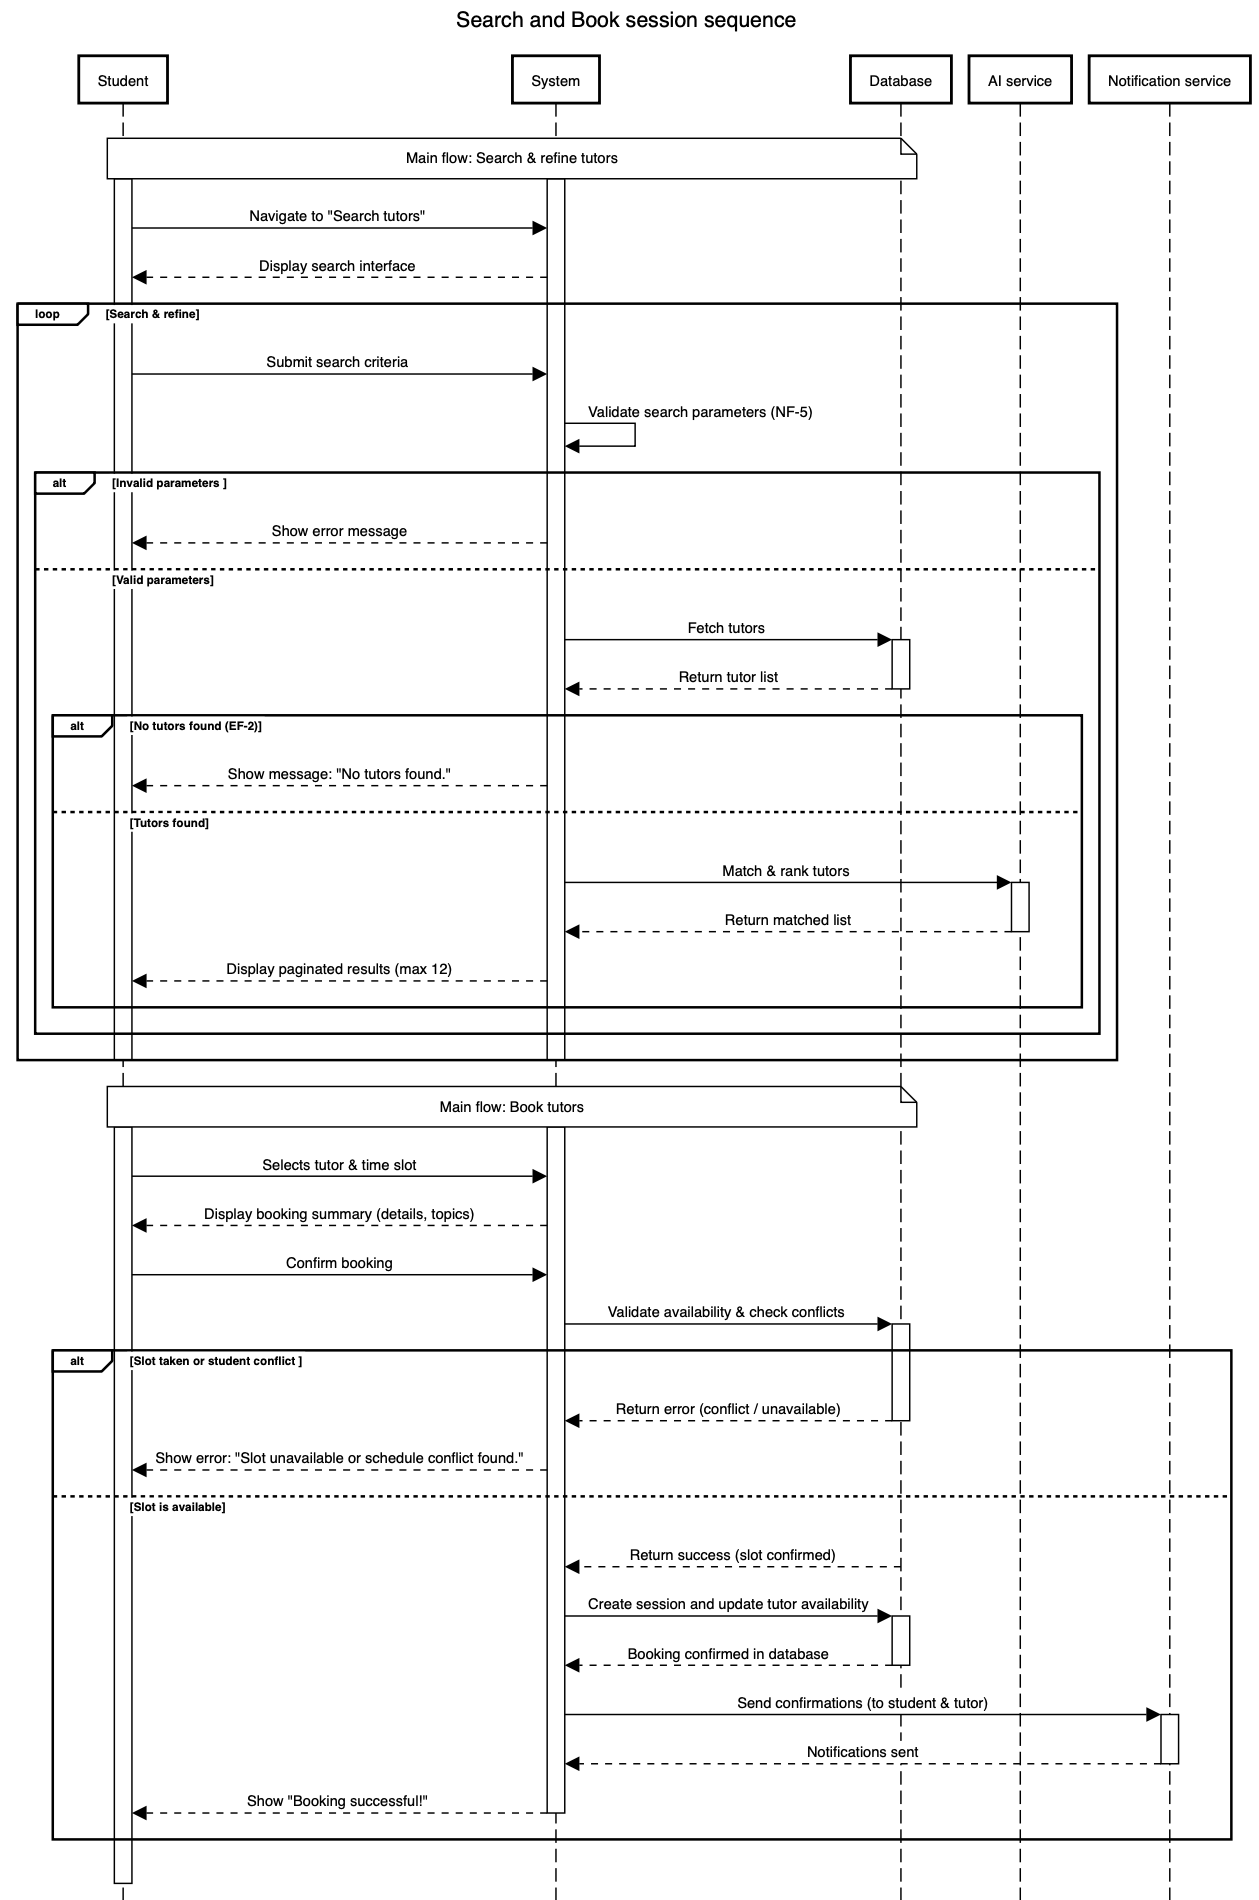
\includegraphics[width=0.7\textwidth]{graphics/chapter3/student/S_B.png}
    \caption{Sequence diagram of Searching and Booking session}
    \label{fig:search and book}
\end{figure}

\noindent \textbf{Description} \\
\textbf{Actors:} Student, System, Database, AI service, Notification service.
\begin{enumerate}
\item Student navigate to searching page and submit theirs criteria.
\item System validates criteria and fetch tutors from database.
\item System send tutor list to AI service for ranking. If no tutors match, system send "No tutors found".
\item System paginated the result to Student.
\item Student selects a tutor, check time slot and confirm booking.
\item If available, System create the session in Database, update that tutor's availability and uses the Notification service to send confirmations.
\item If not (due to schedule conflict or slot taken), System display an error.
\end {enumerate}
